% This chapter will introduce Jupiter's magnetosphere to the reader:
% ------------------------------------------------------------------
\chapter{Introduction}

\section{Fundamentals}


\subsection{The MHD approximation}


The Ohm's law for ideal MHD provides the electric field $\mathbf{E}$ as,
\begin{equation}
    \mathbf{E} = -\mathbf{v} \times \mathbf{B}
\end{equation}

Which states that the electric field perceived by the moving plasma in the frame of reference moving with velocity $\mathbf{v}$ in a background magnetic field $\mathbf{B}$ is zero. Ultimately, this implies the magnetic flux through a surface 

\begin{equation}
    \oint_V \frac{\partial \mathbf{B}}{\partial t} \,dV
\end{equation}

\subsection{Magnetic reconnection}
Magnetic reconnection is a process by which two regions with sufficiently sheared magnetic fields merge and transfer the energy associated with magnetic stresses into the kinetic energy of the surrounding plasma \cite{Priest2000MagneticReconnection,Yamada2010MagneticReconnection}. A simplistic analogy often used to describe magnetic reconnection is the `disconnection' and \emph{re}-connection of two magnetic field lines which are oppositely directed to each other \cite{Gonzalez2016FundamentalReconnection}. Such breakage of magnetic field lines would violate the frozen-in flux condition, and thus, magnetic reconnection is a non-ideal phenomena which requires finite resistivity to occur. 

Figure <> shows a schematic of the region where two regions with anti-parallel magnetic fields merge and reconnect. Magnetic field lines diffuse towards the center of the region, called the `X-line', via the inflow region and are expelled at large velocities away from the X-line in the outflow regions. Various theories have been put forward to explain and model the steady reconnection process, to explain the different rates of observed reconnection (see for e.g. \citeNP{Yamada2010MagneticReconnection} and references therein). In particular, we will discuss the two-fluid model of reconnection. 

In the two-fluid model, the ions and electrons are presumed to demagnetize, i.e. stop following the magnetic field orientation, at different regions near the X-line. The ions, being heavier, are demagnetized first as they enter the \emph{ion diffusion region} and escape via the outflow, where they are accelerated. The electrons remain magnetized until they reach the \emph{electron diffusion region}. The different motions of the electrons and ions generates the quadrupolar Hall magnetic field. As the electron diffusion region is much smaller than those for the ions, it is much difficult to detect in the in-situ measurements and remains an active topic for research. Studying the electron diffusion region was the primary motivation of the MMS spacecraft constellation. 

The model shown in Figure <> represents a situation where magnetic reconnection is occurring in a steady manner. However, particle-in-cell and hybrid simulations of reconnecting fields have shown that this is not necessarily the case. Instead, the thin current sheet near the X-line was found to be unstable to the tearing instability, and breaks into individual closed magnetic loops separated by multiple X-lines \cite{Drake2006ElectronReconnection,Drake2006FormationReconnection}. These magnetic loops, also called flux ropes or O-lines, are created within the ion-diffusion region and are transported away from the X-line through the outflow, where they are free to coalesce through repeated reconnection and enlarge or dissipate \cite{Markidis2012CollisionlessChain,Wang2016CoalescenceReconnection}. 

Magnetic reconnection is a fundamental and ubiquitous process in space plasmas and occurs in most regions of the space environment, from the solar corona to the various planetary magnetospheres, to the heliopause. The implications of magnetic reconnection on the magnetospheres of Earth and Jupiter, and the differences between the two, are discussed in subsequent sections.


\section{Earth's magnetosphere}
A brief description of the processes occurring in the terrestrial magnetosphere is provided in this section to better understand the similarities and differences between it and the Jovian magnetosphere.

\subsection{The solar wind and interplanetary magnetic field}
The solar wind is a stream of particles accompanied by the interplanetary magnetic field (IMF), which flows outward from the sun. It originates from the lower regions of the solar corona, expands and accelerates until it gains a speed roughly between 400 to 600 km/s, by which time it is usually supersonic and super-Alfvenic \cite{Gombosi1998PhysicsEnvironment}. It is composed primarily of protons with an average temperature on the order of $10^5$ K and density of $\sim$7 cm$^{-3}$ (at 1 AU = $1.49 \times 10^{11}$ km), though other species and charge states are also prevalent.

It was hypothesized that the radial flow of solar wind plasma distorts the frozen-in interplanetary magnetic field into a spiral configuration with increasing distance from the sun \cite{Parker1958DynamicsFields.,Ness1964SolarField} (see Figure \ref{fig:parker-spiral}). This may be a reasonable assumption during quiet intervals, but the solar wind and IMF can be highly dynamic, leading to the formation of corotating-interaction-regions (CIRs) and coronal-mass-ejections (CMEs). These can be associated with drastic changes in the solar wind dynamic pressure and orientation of the IMF, which perturbs the terrestrial magnetosphere in various ways \cite{Borovsky2006DifferencesStorms,Denton2006GeomagneticWind}. 

Figure \ref{fig:parker-spiral} shows two interplanetary magnetic field lines which intersect the orbits of Earth and Jupiter at 1 AU and 5.2 AU respectively. The Parker-spiral IMF at Earth possess a large $\mathbf{r}$ component (where $\mathbf{r}$ is the Sun-Earth direction, also the direction of solar wind flow). On the other hand, the IMF is almost fully azimuthal by the time it reaches Jupiter's orbit.

\begin{figure}
    \centering
    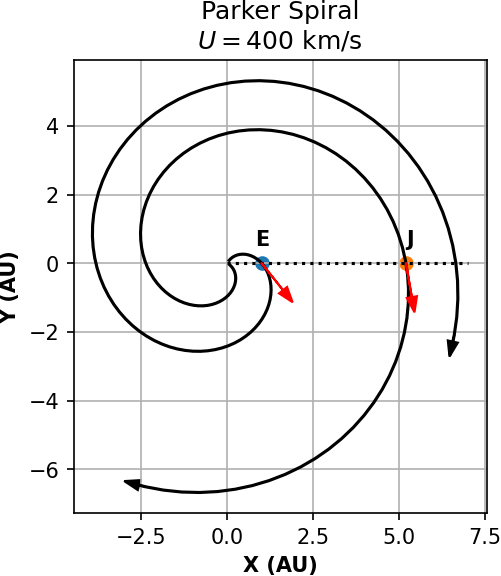
\includegraphics{images1/parker-spiral.png}
    \caption{Interplanetary magnetic field lines showing the Parker-spiral in the ecliptic plane. The field lines intersect at the orbits of Earth and Jupiter at 1 AU and 5.2 AU respectively and the tangent to the curve is highlighted via arrows.}
    \label{fig:parker-spiral}
\end{figure}


\begin{figure}
    \centering
    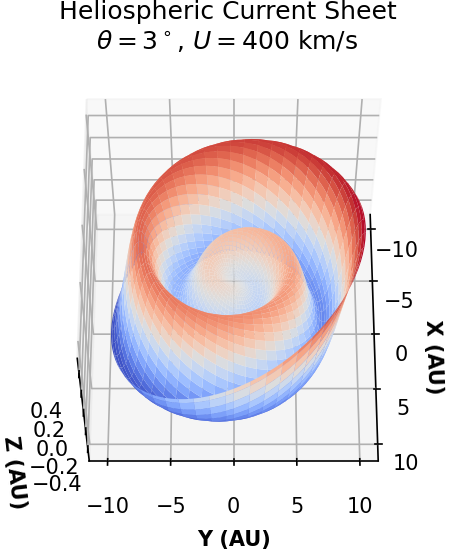
\includegraphics{images1/heliospheric-currentsheet.png}
    \caption{Wavy structure of the heliospheric current sheet assuming a constant 400 km/s solar wind flow and a dipole magnetic field.}
    \label{fig:heliospheric-current-sheet}
\end{figure}


Also associated with the radial outflow of the solar wind is the heliospheric current sheet. Since the solar magnetic axis is not aligned with its spin axis, the heliospheric current sheet undulates about a mean position at the Equator (Figure \ref{fig:heliospheric-current-sheet}). At Earth, this can be seen in the North-South ($Z$) component of the IMF. Periods when the IMF is southward, and thus oppositely directed to the planetary field at the dayside boundaries of the magnetosphere, are considered to lead to increased geomagnetic activity due to magnetic reconnection (discussed in later sections). 

\subsection{Configuration of the terrestrial magnetosphere}
The interaction between the solar wind and interplanetary magnetic field with the internal magnetic field of the Earth forms the magnetosphere. Since the incoming plasma is supersonic and super-Alfvenic, a bow shock is created at the interaction front. Downstream of the shock lies a region of shocked high-temperature solar wind called the magnetosheath. The magnetic field strength in the magnetosheath is larger than in the solar wind, but the field lines are still `open', i.e. they are connected at both ends to the interplanetary magnetic field. Separating the planetary field from the magnetosheath is a discontinuity called the magnetopause. The magnetopause is a current layer that shields the magnetosphere from the external inputs.

On the nightside, the interaction of the tail magnetic field with the solar wind and IMF creates a magnetotail. Magnetic field lines in the magnetotail are considered to be primarily in the plane of the solar wind flow. Present between oppositely directed magnetic field lines in the northern and southern magnetotail lobes is the magnetospheric tail current sheet, which is surrounded by a region of high-density plasma called the plasmasheet. 

In the inner regions of the magnetosphere are the planet's radiation belts - regions of trapped high-energy particles undergoing repeated bounce motions. In these regions the current sheet is weak or non-existent and the magnetic field is close to being dipolar. Co-located with the radiation belts is the plasmasphere, composed of relatively low-energy particles (ions and electrons) which are undergoing the $\mathbf{E}\times\mathbf{B}$ drift in the planetary field.

\subsection{Magnetic reconnection in the terrestrial magnetosphere}
In the context of the terrestrial magnetosphere, magnetic reconnection is usually studied in two regions. The first region is the dayside magnetopause, where high density plasma of the magnetosheath associated with a strong magnetic field interacts with the relatively low density plasma of the magnetosphere, associated with weaker magnetic fields. Magnetic reconnection has been observed to occur at all orientations of the IMF (clock angle), but is most prominent when the IMF is pointing southward, as in this situation the magnetic shear between it and the northward pointing magnetospheric field (at the magnetopause) is maximized. In such a case, `open' field lines in the solar wind reconnect with `closed' field lines of the magnetosphere, and produce newly opened field lines which are transported away from the reconnection site by the reconnection outflow.

The second region where reconnection is studied widely is the terrestrial magnetotail. Magnetic field lines in the northern and southern magnetotail lobes which are separated by the magnetotail current sheet are often directed oppositely to one another. Two such open field lines in the magnetotail may spontaneously reconnect and convert into a single closed field line. More often, magnetic reconnection is observed to occur near the planet, where field lines may still be closed, and is preceded by a thinning of the magnetotail current sheet, and results in an explosive reconnection event called a \emph{substorm}. 

\subsection{Ionosphere}
Neutral species in Earth's upper atmosphere are photo-ionized, and the relatively low-densities at higher altitudes lead to longer collision time scales which supports a persistent region of charged particles called the ionosphere. Being full of ions and electrons, the highly conducting ionosphere is intricately connected with the magnetosphere.

Ionospheric plasma at mid- to low-latitudes corotates with the planet due to collisions with the corotating thermospheric neutrals. The magnetic field lines associated with these regions are connected at both ends with the planet (i.e. they are \emph{closed}) and have an equatorial footprint in the magnetosphere at a distance of a few Earth radii. Since the field lines in ideal MHD can be considered to possess the same electrostatic potential, the corotation velocity of the ionospheric plasma is transmitted to the associated magnetic flux tube in the magnetosphere. This creates a corotating region of low-energy plasma called the plasmasphere. This picture is consistent with the argument that the plasmasphere is a result of $\mathbf{E}\times\mathbf{B}$ drift, where $\mathbf{E}=-\nabla \Phi$ can be considered to be the corotation electric field. Thus, the ionosphere plays a crucial role in maintaining the corotation at Earth. 

At higher latitudes, magnetic field lines are open, i.e. they are connected at one end with the interplanetary magnetic field. In such a case, the ionosphere plays a more responsive role to changes in the solar wind and distant magnetosphere. 

Field aligned currents from the magnetosphere close through perpendicular (to $\mathbf{B}$) currents in the ionosphere. 






\subsection{Magnetosphere-ionosphere coupling}


\section{Jupiter's magnetosphere}


\subsection{The inner magnetosphere}
The large natural satellites of the gas giants greatly contribute to plasma dynamics in their magnetospheres. At Jupiter, the largest moons in increasing order of radial distance from the planet are Io, Europa and Ganymede. Out of these, Io and Europa and considered to be un-magnetized, but interact with the surrounding magnetospheric plasma due to the resistive effects of subsurface magma and saline oceans respectively. Ganymede is the only known natural satellite in the solar system which possess a strong internal magnetic field, which interacts with the Jovian magnetic field to create its own magnetosphere. 

Out of these satellites, Io and Europa are responsible for contributing substantial mass to the inner magnetosphere of Jupiter. Volcanism at Io creates SO$_2$, which is ionized either via photo-ionization or electron-impact ionization to produce S$^{++}$, O$^+$ etc. Meanwhile, plumes at Europa eject water neutrals into the surroundings, which ionize to produce water group ions - H$^+$, O$^+$ etc. the net contribution of this ionization results in a mass addition of approximately 250-1000 kg/s for Io and 50 kg/s for Europa. A similar situation is seen at Saturn, where Enceladus adds $\sim$50 kg/s to its magnetosphere. Local loss mechanisms at such as charge exchange cannot fully account for this addition of mass. 

The newly created ions are ``picked-up'' by the surrounding magnetospheric plasma. Newly created plasma ions, which presumably still possess the Keplerian velocity of the neutrals ($\sim$10 km/s at Io's orbit), perceive the motional electric field ($\mathbf{E} = -\mathbf{u} \times \mathbf{B}$) due to the faster magnetospheric flow ($u=\sim200$ km/s) and undergo the $\mathbf{E} \times \mathbf{B}$ drift. Ion pickup increases particle velocity in the direction perpendicular to the magnetic field, increasing anisotropy. 

The magnetospheric plasma in the inner magnetosphere corotates with the planet. Corotation at these distances is facilitated through ion-neutral collisions in the Jovian ionosphere, which prevents a velocity gradient from forming between the thermosphere and ionosphere. The ionosphere then transmits the velocity to all regions in the magnetosphere with which it is connected via magnetic field lines. The corotation process in the inner magnetosphere does not require the presence of large-scale field aligned currents as in the case of the middle and outer magnetosphere, which we will discuss in the next section. 

\subsection{The middle magnetosphere}
The plasma created in the inner magnetosphere of Jupiter is believed to be lost through a series of instabilities. The large density in the inner magnetosphere leads to a decrease in flux tube content with radial distance, which, in the presence of the centrifugal force, creates regions unstable to the interchange instability. Observations by the Galileo and Cassini spacecraft have detected plasma and magnetic signatures containing pockets of high magnetic field strength or high energy plasma which is lower in density, within regions of low energy, high-density plasma. 

It is believed that as Iogenic plasma moves from the inner magnetosphere to further radial distances, the conservation of angular momentum results in the loss of its azimuthal velocity. The slowing down of magnetospheric plasma creates a ``bend-back'' of the frozen-in magnetic field lines in the equatorial plane. The bending of these field lines, or more accurately, the production of magnetic curvature, creates radial currents in the equatorial region to counter the deceleration due to angular-momentum conservation. The radial currents, together with the predominantly southward magnetic field, create a $\mathbf{J}\times\mathbf{B}$ force in the azimuthal direction. These ``corotation-enforcement'' currents are closed via field-aligned currents and perpendicular currents in the Jovian ionosphere. The ionospheric location corresponding to the outward currents (and hence, precipitating electrons) is considered to be the location of the main oval of the Jovian ultraviolet aurora.

The centrifugal force in Jupiter's magnetosphere also stresses the field in the radial direction, leading to the formation of a `magnetodisc' configuration and a strong cross tail current sheet. Evidence for this process has been provided by in-situ spacecraft such as Galileo and Juno, which observed that field lines located at large distances departed greatly from the dipole expectation. 

\subsection{The outer magnetosphere}
Eventually, the stretching of magnetic field lines at large radial distances on the nightside thins the equatorial current sheet to an extent that allows for magnetic reconnection to take place. Reconnection in Jupiter's magnetosphere is different from the Dungey-cycle reconnection seen in the terrestrial magnetosphere, where open field lines in the magnetotail reconnect and produce a closed field line. At Jupiter, magnetotail reconnection is believed to occur spontaneously due to the thinning of the magnetotail current sheet, leading to reconnection within the same field line. This process detaches a loop-like magnetic structure which is disconnected from the other closed field lines and is free to travel tailward and escape the magnetosphere. Since these loop-like structures transport plasma away from the magnetosphere, they are referred to as ``plasmoids''. The newly reconnected closed field line, now devoid of heavy mass, returns to the planet and continues to corotate and get loaded with mass from the inner magnetosphere. This cycle of mass loss through internal magnetic reconnection is called the ``Vasyliunas'' cycle. The Vasyliunas cycle is considered to be the final process that facilitates the loss of Iogenic plasma from the magnetosphere to the external solar wind.

In-situ observations by Galileo and Juno have shown that plasmoids are created in the Jovian magnetosphere due to magnetic reconnection. The observed plasmoids were fairly large, with diameters ranging between 2-20 $R_J$. Despite their size, it was estimated that the mass carried by theses plasmoids could account for an effective loss of ~200 kg/s, much less than the ~1000 kg/s added by Io. 


\section{Solar wind conditions at Jupiter}

\section{Jupiter's UV aurora}

\section{Objectives of this study}d

% \section{Open questions}
% \subsection{Variability of the Jovian UV aurora: Effect of solar wind dynamic pressure?}
% \subsection{Does Dungey-cycle reconnection play an important role?}
% \subsection{How is plasma }

